\chapter{Introduction to Gravitational Lensing}

One of the most amazing results of Einstein's theory of general relativity, regarding the distortion of space time by massive objects is gravitational lensing. The basic principle behind gravitational lensing is that light is distorted when it travels close to the potential well (the distortion of space time) of massive objects (analogous to the effect of optical lenses). Under certain conditions the background objects can be seen in multiple images and ``arcs" surrounding the lensing object, this is known as strong gravitational lensing. 

For the general lens we first start by introducing the deflection angle which is the measure of the angular distance that has been deflected and which is linearly dependent on the mass $M$. This dependence ensures that the angles of deflection of an array of lenses can be superposed linearly. If we had N point masses sparsed one a plane, with positions $\xi$ and masses $M_{i}$, then the deflection angle would be:

equation 1

Fortunately, in most three dimensional distributions of matter (even in the case of lensing by massive objects like galaxy clusters) the physical size of the lens is generally much smaller than the distances between the observer, the lens and the source. This means that the deflection of light takes place in a very thin and short section of its path to the observer. Given this, we can use the \textit{thin screen approximation}: "The lens is approximated by a planar distribution of matter, the lens plane". Also the sources can be treated as if they lie on a plane which is called the source plane.

The \textit{thin screen approximation} allows us to state that the lensing matter distribution is fully described by its surface density

equation 2

where $\vec{\xi}$ is a two-dimensional vector on the lens plane and $\rho$ is the three dimensional density.

\begin{figure}[H]
\centering
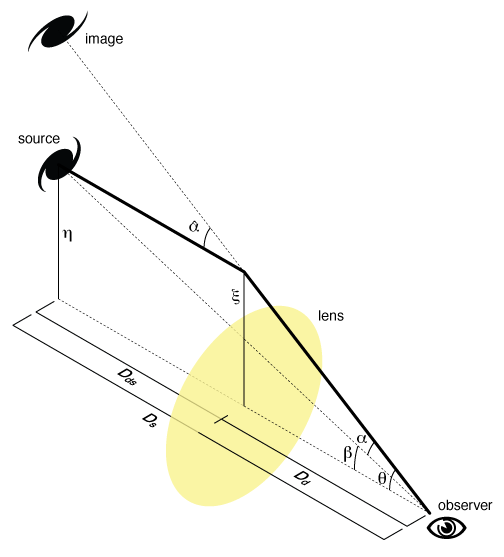
\includegraphics[width=12cm]{images/lensing.png}
\caption[Angles in gravitational lensing]{where $D_{ds}$ is the distance from the lense to the source $D_s$ is the distance from the observer to the source and $D_d$ is the distance from the observer to the source Wikipedia}
\end{figure}

Figure [] is a sketch of a typical gravitational system. The lensing mass is located at a angular diameter distance $D_d$ and it deflects the light rays coming from a source at an angular distance of $D_s$.

The optical axis is perpendicular to the lens and source planes and passes through the observer. We measure the angular positions on both planes with respect to this reference direction. The source is at the angular position $\vec{\beta}$ and lies on the source plane at a distance $\vec{\eta}=\vec{\beta}D_s$ from the optical axis. The deflection angle $\hat{\vec{\alpha}}$ of the light ray comes from the source and has impact parameter $\vec{\xi}=\vec{\theta}D_d$ on the lens plane. Due to this deflection, the observer receives the light coming from the source as if it was emitted at the angular position $\vec{\theta}$.

If $\vec{\theta}$, $\vec{\beta}$ and $\hat{\vec{\alpha}}$ are small, the true position of the source and its observed position on the sky are related by a very simple relation, obtained by a geometrical construction. This relation is called the lens equation and is written as

\begin{equation}
\vec{\theta}D_s = \vec{\beta}D_s+ \hat{\vec{\alpha}}D_{ds}     \\\\\\\\\\\
\end{equation}

where as seen in the figure, $D_{ds}$ is the distance between the lens and the source.

Defining the reduced deflection angle

\begin{equation}
\vec{\alpha}(\vec{\theta})\equiv \frac{D_{ds}}{D_s}\hat{\vec{\alpha}}(\vec{\theta})
\end{equation}

From equation ..... we get

\begin{equation}
\vec{\beta}=\vec{\theta}-\vec{\alpha}(\vec{\theta})
\end{equation}

The most interesting physics of the simple lens equation arises because $\vec{\alpha}$ depends on $\vec{\theta}$

Now, we can characterize an extender distribution of matter by it effective lensing potential, which is obtained by projecting the three-dimensional Newtonian potential on the lens plane and scaling it accordingly

\begin{equation}
\hat{\Psi}(\vec{\theta})=\frac{D_{ds}}{D_{d}D_{s}}\frac{2}{c^{2}}\int\Phi(D_{d}\vec{\theta},z)dz
\end{equation}

This lensing potential satisfies two important properties:

1) the gradient of $\Psi$ gives the scaled deflection angle:

\begin{equation}
\vec{\nabla}_{x}\Psi(\vec{x})=\vec{\alpha}(\vec{x})
\end{equation}

2) the Laplacian of $\varPsi$ gives twice the convergence

\begin{equation}
\Delta_{x}\Psi(\vec{x})=2\kappa(\vec{x})
\end{equation}

where the convergence is defined as a dimensionless surface density

\begin{equation}
\kappa(\vec{x})\equiv \frac{\Sigma(\vec{x})}{\Sigma_{cr}}\qquad \text{with} \qquad \Sigma_{cr}=\frac{c^{2}}{4\pi G}\frac{D_s}{D_d D_{ds}}
\end{equation}

$\Sigma_{cr}$ is called the critical surface density and it characterises the lens system and which is a function of the angular diameter distances of lens and source. 

Now let's talk about magnification and distortion.

One of the main features of gravitational lensing is that it distorts the shapes of the sources, this is particularly evident when the source has no negligible apparent size. In some cases the background galaxies can appear as very long arcs in galaxy clusters as mentioned at the beginning of this chapter. 

desde aca hay que modificar!!!!!!!!!!


The distortion takes place because light bundles are deflected differentially. Ideally the shape of the images can be determined by solving the lens equation for all the points within the extended source. In particular, if the source is much smaller than the angular size on which the physical properties of the lens change, the relation between the source and image positions can locally be linearised. In other words, the distortion of images can be described by the Jacobian matrix
\begin{equation}
A\equiv\frac{\partial\vec{y}}{\partial\vec{x}}=\left(\delta_{ij}-\frac{\partial\alpha_{i}(\vec{x})}{\partial x_{j}}\right)=\left(\delta_{ij}-\frac{\partial^{2}\Psi(\vec{x})}{\partial x_{i}\partial x_{j}}\right)
\end{equation}

where $x_i$ indicates the $i$-component of $\vec{x}$ on the lens plane. it shows that the elements of the Jacobian matrix can be written as combinations of the second derivatives of the lensing potential. For brevity, we will use the shorthand notation

\begin{equation}
\frac{\partial^{2}\Psi(\vec{x})}{\partial x_{i}\partial x_{j}}\equiv\Psi_{ij}
\end{equation}

We can now split off an isotropic part from the Jacobian:

\begin{equation}
\left(A-\frac{1}{2}trA\cdot I\right)_{ij}=\left(\begin{array}{cc}
-\frac{1}{2}\left(\Psi_{11}-\Psi_{22}\right) & -\Psi_{12}\\
-\Psi_{12} & \frac{1}{2}\left(\Psi_{11}-\Psi_{22}\right)
\end{array}\right)
\end{equation}

which is an antisymmetric, trace-free matrix called the shear matrix. It quantifies the projection of the gravitational tidal field (the gradient of the gravitational force), which describes distortions of background sources.  This allows us to define the pseudo-vector $\vec{\gamma}=(\gamma_1 , \gamma_2)$ on the lens plane, whose components are

\begin{equation}
\gamma_1(\vec{x})=\frac{1}{2}(\Psi_{11}-\Psi_{22})\qquad and \qquad \gamma_2(\vec{x})=\Psi_{12} = \Psi_{21}
\end{equation}

This is called the shear. The eigenvalues of the shear matrix are 

\begin{equation}
\pm \sqrt{\gamma_1^2 + \gamma_2^2} = \pm \gamma
\end{equation}

Thus, there exists a coordinate rotation by an angle $\phi$ such that 

\begin{equation}
\left(\begin{array}{cc}
\gamma_{1} & \gamma_{2}\\
\gamma_{2} & -\gamma_{1}
\end{array}\right)=\gamma\left(\begin{array}{cc}
\cos2\phi & \sin2\phi\\
\sin2\phi & -\cos2\phi
\end{array}\right)
\end{equation}

And for the trace we have

\begin{equation}
\frac{1}{2}trA=(1-\kappa)\delta_{ij}
\end{equation}

This the Jacobian becomes 

\begin{equation}
A= \left(\begin{array}{cc}
1-\kappa-\gamma_{1} & -\gamma_{2}\\
-\gamma_{2} & 1-\kappa+\gamma_{1}
\end{array}\right)
\end{equation}

Where $\kappa$ is the convergence that determines the magnification and $\gamma_{1}$ and $\gamma_{2}$ are the shear components that determine the distortion of the background objects. This is an antisymmetric, trace-free matrix that quantifies the projection of the gravitational tidal field (the gradient of the gravitational force), which describes distortions of background sources.

Finally, we can introduce another useful quantity in the characterization of gravitational lensing systems. The \textit{magnification} is quantified by the inverse of the determinant of the Jacobian matrix. For this reason, the matrix $M=A^{-1}$ is called the \textit{magnification tensor}, and we define

\begin{equation}
\mu \equiv \text{det} M = \frac{1}{\text{det}A}=\frac{1}{(1-\kappa)^2-\gamma^2}
\end{equation}

The eigenvalues of the magnification tensor measure the amplification in the tangential and in the radial direction and are given by

\begin{equation}
\mu_t = \frac{1}{\lambda_t}=\frac{1}{1-\kappa - \gamma} \qquad and \qquad  \mu_r = \frac{1}{\lambda_r}=\frac{1}{1-\kappa + \gamma}
\end{equation}

The magnification is ideally infinite where $\lambda_t=0$ and where $\lambda_r=0$. These two conditions define two curves in the lens plane, called the tangential and the radial critical line, respectively. An image forming along the tangential critical line is strongly distorted tangentially to this line. On the other hand, an image forming close to the radial critical line is stretched in the direction perpendicular to the line itself. 

There are three classes of gravitational lensing:

1. \textbf{Strong lensing:} where there are easily visible distortions such as the formation of Einstein rings, arcs, and multiple images.

2.\textbf{ Weak lensing:} where the distortions of background sources are much smaller and can only be detected by analysing large numbers of sources in a statistical way to find coherent distortions of only a few percent

3. \textbf{Very weak lensing:} 

\begin{figure}[H]
\centering
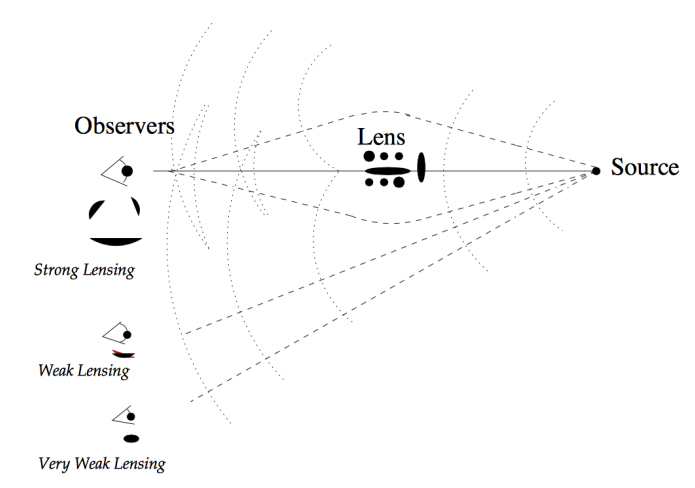
\includegraphics[width=12cm]{images/types_of_lensing.png}
\caption[Types of lensing]{Types of lensing. Courbin, F. et al \citeyear{Reference24}}
\end{figure}

Figure [] is a representation of a lensing system in which a background galaxy is lensed by a cluster of galaxies and produces multiple images as observed from Earth. 

\begin{figure}[H]
\centering
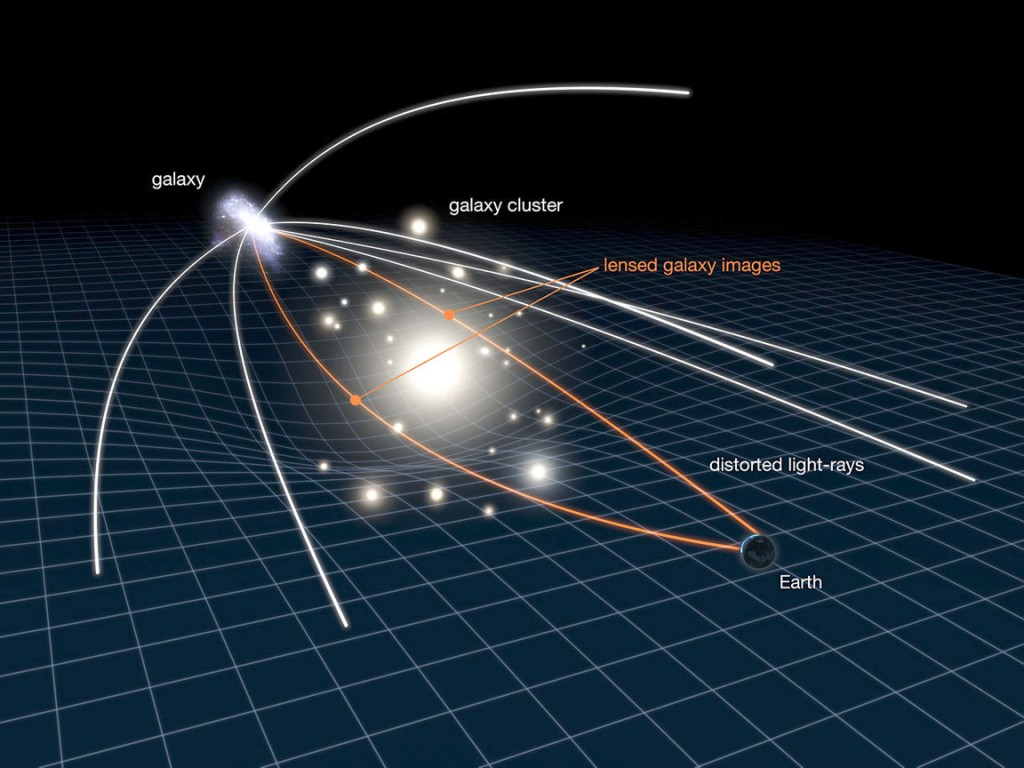
\includegraphics[width=12cm]{images/strong_lensing.jpg}
\caption[Strong Lensing representation]{Nasa?}
\end{figure}

Figure [] is a composite image of a galaxy cluster taken by the HST in which many lensed objects can be seen as distorted shapes and multiple images. 

\begin{figure}[H]
\centering
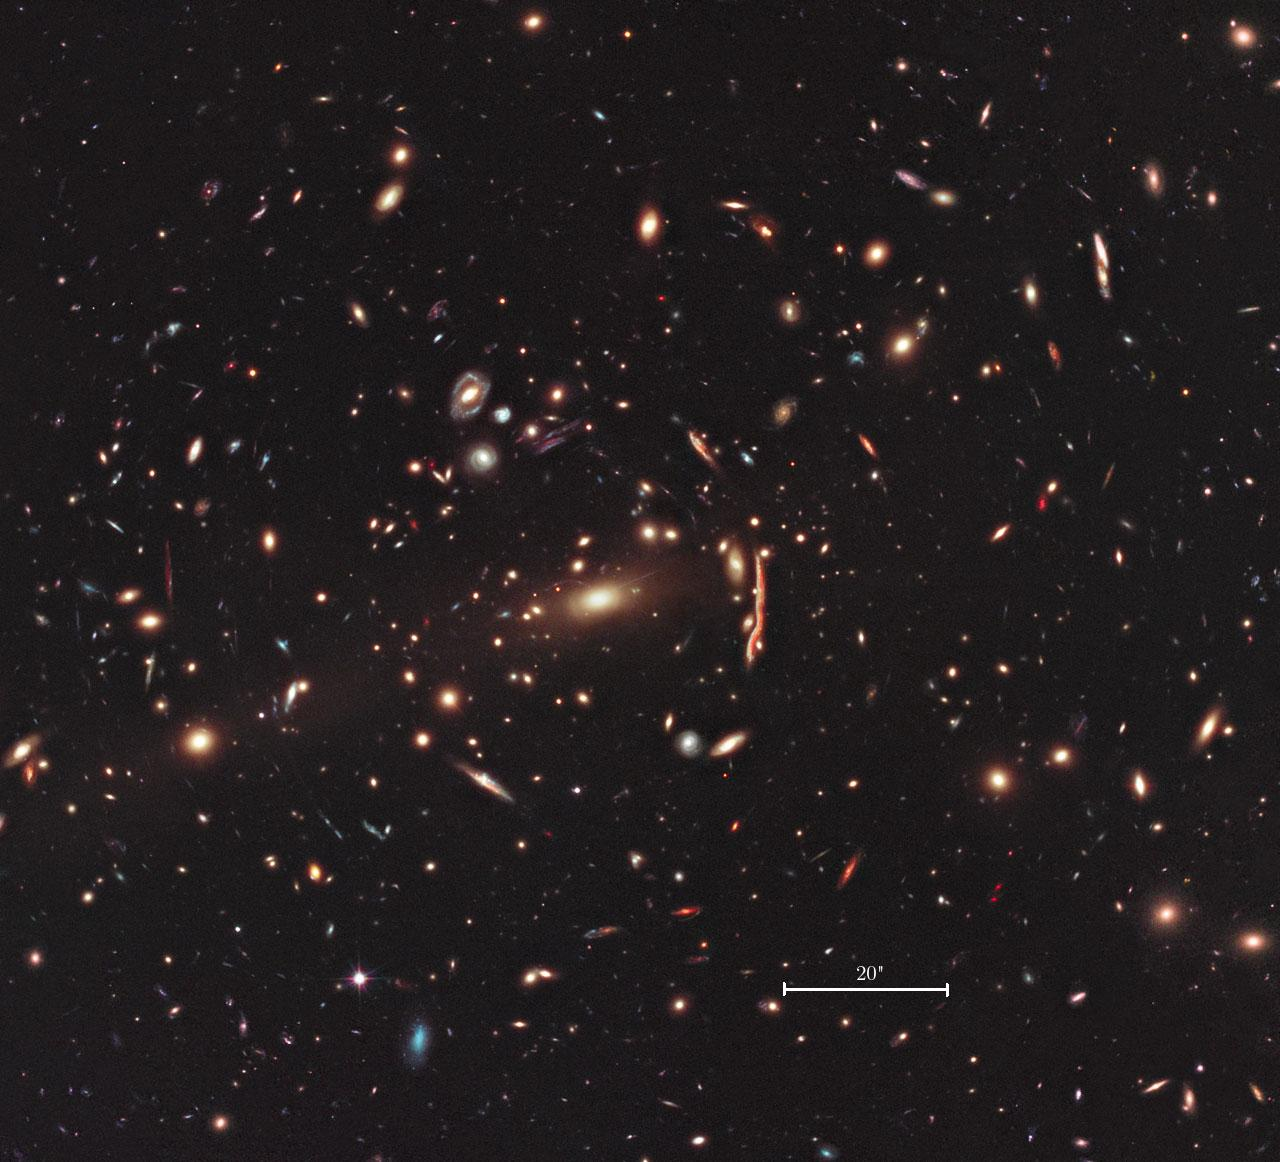
\includegraphics[width=12cm]{images/GC.jpg}
\caption[Galaxy Cluster MACS 1206]{Galaxy Cluster MACS 1206, credits to NASA Hubble Space Telescope}
\end{figure}

Quoted (need to change this): The image of galaxy cluster MACS J1206.2-0847 (or MACS 1206) is part of a broad survey with NASA Hubble Space Telescope. The distorted shapes in the cluster are distant galaxies from which the light is bent by the gravitational pull of an invisible material called dark matter within the cluster of galaxies. This cluster is an early target in a survey that will allow astronomers to construct the most detailed dark matter maps of more galaxy clusters than ever before.These maps are being used to test previous, but surprising, results that suggest that dark matter is more densely packed inside clusters than some models predict. This might mean that galaxy cluster assembly began earlier than commonly thought.

Scientists are planning to observe a total of 25 galaxy clusters under a project called CLASH (Cluster Lensing and Supernova survey with Hubble). One of the first objects observed for the new census is the galaxy cluster MACS J1206.2-0847. This conglomeration of galaxies is one of the most massive structures in the universe, and its gigantic gravitational pull causes stunning gravitational lensing. MACS 1206 lies 4 billion light-years from Earth. In addition to curving of light, gravitational lensing often produces double images of the same galaxy. In the new observation of cluster MACS J1206.2-0847, astronomers counted 47 multiple images of 12 newly identified galaxies.The era when the first clusters formed is not precisely known, but is estimated to be at least 9 billion years ago and possibly as far back as 12 billion years ago. If most of the clusters in the CLASH survey are found to have excessively high accumulations of dark matter in their central cores, then it may yield new clues to the early stages in the origin of structure in the universe.

Galaxies and clusters of galaxies that act as gravitational lenses can be approximated by single isothermal spheres. It is easy to relate an angular scaling parameter $\xi_{E}$, referred to as the Einstein radius, to the mass inside the corresponding light cone. The Einstein radius corresponds to the ring image of a point source aligned exactly on the axis of the lens.

Summary of isothermal sphere:

\begin{equation}
\rho(r)=\frac{\sigma^2}{2\pi Gr^2}
\end{equation}

\begin{equation}
\Sigma(\xi)=\frac{\sigma^2}{2G\xi}
\end{equation}

\begin{equation}
\xi_{E}=4\pi\left(\frac{\sigma}{c}\right)^{2}\frac{D_{ds}}{D_{s}}
\end{equation}

In reality, the density profile and lensing properties of galaxies is a bit more complicated than the assumption of a singular isothermal sphere, so we need to take into account more complex but elaborate profiles such as the NFW (Navarro, Frenk, White, \citeyear{Reference17}).

The NFW density profile is 

\begin{equation}
\rho(r)=\frac{\delta_{c}\rho_{c}}{(r/r_{s})(1+r/r_{s})^{2}}
\end{equation}

where the characteristic over density (dimensionless quantity) is given by:

\begin{equation}
\delta_{c}=\frac{200}{3}\frac{c^{3}}{\ln{(1+c)}-c/(1+c)}
\end{equation}

The mass of an NFW halo contained within a radius of $r_{200}$ is:

\begin{equation}
\text{M}_{200}=\text{M}(r_{200})=\frac{800\pi}{3}\rho_{c}r^{3}_{200}=\frac{800\pi}{3}\frac{\bar{\rho}(z)}{\Omega(z)}r^{3}_{200}
\end{equation}

The concentration parameter $c$ is strongly correlated with Hubble type, c=2.6 separating early from late-type galaxies. Those galaxies with concentration indices $c>2.6$ are early-type galaxies reflecting the fact that the light is more concentrated towards their centres, its formal definition in terms of the virial and characteristic radius is $c=r_{200}/r_{s}$.

Dutton \& Maccio \citeyear{Reference23} (in continuation of previous studies such as Mu\~noz Cuartas et. al. \citeyear{Reference12}), made simulations of halo masses from dwarf galaxies to galaxy clusters and find constraints on the concentration parameter for different redshifts, the relation between the concentration parameter with redshift and virial mass is shown in figure [].

\begin{figure}[H]
\centering
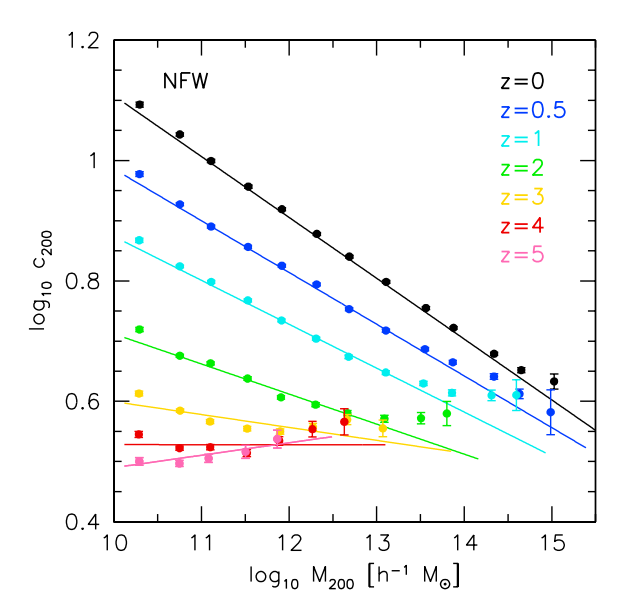
\includegraphics[width=10cm]{images/dutton.png}
\caption[Evolution of the concentration mass relation]{Evolution of the concentration mass relation, by Dutton \& Maccio, \citeyear{Reference23}}
\end{figure}

The surface mass density in the NFW profile is given by:

\begin{equation}
\Sigma_{\text{NFW}}(x) = \left\lbrace
\begin{array}{lll}
\frac{2r_{s}\delta_{c}\rho_{c}}{\left(x^{2}-1\right)}\left[1-\frac{2}{\sqrt{1-x^{2}}}\arctanh\sqrt{\frac{1-x}{1+x}}\right] & (x<1)\\\\
\frac{2r_{s}\delta_{c}\rho_{c}}{3} & (x=1)\\\\
\frac{2r_{s}\delta_{c}\rho_{c}}{\left(x^{2}-1\right)}\left[1-\frac{2}{\sqrt{x^{2}-1}}\arctan\sqrt{\frac{x-1}{1+x}}\right] & (x>1)
\end{array}
\right.
\end{equation} 

so from the critical density:

\begin{equation}
\rho_{c}=\frac{3H^2(z)}{8\pi G}
\end{equation}

$H(z)=H_{0}(1+\Omega z)^{3/2}$

But we are more interested in the enclosed mass which can be done by integrating the surface mass density:

\begin{equation}
\text{M}(R)=\int_{0}^{R}2\pi R\Sigma(R)dR
\end{equation}

The radial dependence on the shear is:

\begin{equation}
\gamma_{\text{NFW}}(x) = \left\lbrace
\begin{array}{lll}
\frac{r_{s}\delta_{c}\rho_{c}}{\Sigma_c}g_{<}(x) & (x<1)\\\\
\frac{r_{s}\delta_{c}\rho_{c}}{\Sigma_c}\left[\frac{10}{3}+4 \ln \left(\frac{1}{2}\right)\right] & (x=1)\\\\
\frac{r_{s}\delta_{c}\rho_{c}}{\Sigma_c}g_{>}(x) & (x>1)
\end{array}
\right.
\end{equation} 

where: 

\begin{equation}
g_{<}(x)=\frac{8 \arctanh \sqrt{\frac{1-x}{1+x}}}{x^{2}\sqrt{1-x^{2}}}+\frac{4}{x^{2}} \ln \left(\frac{x}{2}\right)-\frac{2}{\left(x^{2}-1\right)}+\frac{4 \arctanh \sqrt{\frac{1-x}{1+x}}}{\left(x^{2}-1\right)\left(1-x^{2}\right)^{1/2}}
\end{equation}

\begin{equation}
g_{<}(x)=\frac{8 \arctan \sqrt{\frac{x-1}{1+x}}}{x^{2}\sqrt{x^{2}-1}}+\frac{4}{x^{2}}\ln \left(\frac{x}{2}\right)-\frac{2}{\left(x^{2}-1\right)}+\frac{4 \arctan \sqrt{\frac{x-1}{1+x}}}{\left(x^{2}-1\right){}^{3/2}}
\end{equation} 

and with the critical surface mass density:

\begin{equation}
\Sigma_{c}\equiv\frac{c^{2}}{4\pi G}\frac{D_{s}}{D_{d}D_{ds}}
\end{equation}

these equations come from the paper Wright and Brainerd 1999.

The magnification tensor is:

\begin{equation}
\frac{\partial\beta}{\partial\theta}=\delta_{ij}-\frac{\partial^{2}\psi}{\partial\theta_{i}\partial\theta_{j}}=\left(\begin{array}{cc}
1-\kappa-\gamma_{1} & -\gamma_{2}\\
-\gamma_{2} & 1-\kappa+\gamma_{1}
\end{array}\right)
\end{equation}

The total magnification $\mu$ is given by the determinant of the magnification tensor:

\begin{equation}
\mu = \frac{1}{(1-\kappa)^{2}-\gamma^{2}_{1}-\gamma^{2}_{2}}
\end{equation}



